\addcontentsline{toc}{chapter}{Занятие 12. Проверка параметрических гипотез.
                              Критерий Неймана-Пирсона}
\chapter*{Занятие 12. Проверка параметрических гипотез. Критерий Неймана-Пирсона}

\addcontentsline{toc}{section}{Контрольные вопросы и задания}
\section*{Контрольные вопросы и задания}

\subsubsection*{Что называется статистической гипотезой?}

Статистическая гипотеза --- предположение о виде распределения и свойствах случайной величины,
которое можно подтвердить или опровергнуть применением статистических методов к данным выборки.

\subsubsection*{Какую гипотезу называют основной, альтернативной, простой, сложной?}

Нулевая гипотеза --- гипотеза, подлежащая проверке.
Альтернативная гипотеза --- каждая допустимая гипотеза, отличная от нулевой.
Нулевую гипотезу обозначают $H_0$, альтернативную ---
$H_1$ (от Hypothesis --- <<гипотеза>> (англ.)).

Простой гипотезой называют предположение, состоящее в том,
что неизвестная функция $F \left( t \right) $
отвечает некоторому совершенно конкретному вероятностному распределению.

Сложной гипотезой называют предположение о том,
что неизвестная функция $F \left( t \right) $ принадлежит некоторому множеству распределений,
состоящему из более чем одного элемента.

\subsubsection*{Что такое статистический критерий?}

Статистический критерий --- строгое математическое правило,
по которому принимается или отвергается та или иная статистическая
гипотеза с известным уровнем значимости.

\subsubsection*{Что такое уровень занчимости критерия для проверки статистической гипотезы?}

Можно отвергнуть гипотезу $F_1$, когда она будет верна.
В случае простой гипотезы $F_1$ вероятность ошибки равна  $P_{F_1} \left( \vec{X} \in D \right) $.
Эту вероятность называют уровнем значимости статистического критерия.

\subsubsection*{Какое множество называют критическим для проверки статистической гипотезы?}

Критическая область --- это совокупность значений статистики, которые <<говорят>>,
что нулевую гипотезу следует отвергнуть.

\subsubsection*{В чём состоит ошибка первого рода, второго рода?}

$1 - \alpha = P \left( H_1 \; \middle| \; H_0 \right) $ --- ошибка первого рода.
Означает, что отклонили нулевую гипотезу в то время, как на самом деле она истинна.

$ \beta = P \left( H_0 \; \middle| \; H_1 \right) $ --- ошибка второго рода.
Это означает принять нулевую гипотезу, которая на самом деле ложна.

\subsubsection*{Что называют мощностью критерия?}

$1 - \beta $ --- мощность критерия.

\subsubsection*{Сформулируйте критерий согласованности Колмогорова,
                критерий согласованности $ \chi^2$ Пирсона, лемму Неймана-Пирсона}

\textit{Критерий Колмогорова-Смирнова.}
Если $F$ --- непрерывное распределение,
то
$ \sqrt{n} \cdot
  \sup \limits_{ \mathbb{R}} \left[ F_n \left( x \right) - F \left( x \right) \right] \approx
  D_{ \theta }$
--- известное распределение.

\textit{Критерий Пирсона (критерий согласия $ \chi^2$).} Есть выборка $X_1, \dotsc, X_n$.
Имеет ли оа распределение $F$?
Попробуем устроить дискретную процедуру.
Разбиваем интервал возможных значений выборки на $N$ полуинтервалов (чисел, частей) ---
рис. \ref{fig:12}.

\begin{figure}[h!]
  \centering
  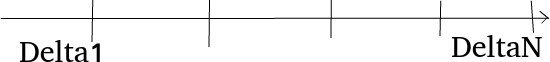
\includegraphics[width=.4\textwidth]{./pictures/12.png}
  \caption{Возможные значения выборки}
  \label{fig:12}
\end{figure}

Обозначим через $p_i = P_F \left( X_1 \in \Delta_i \right) > 0$.

Количество элементов выборки, которые попали в $ \Delta_i$, обозначим через
$$ \nu_i =
  \sum \limits_{k = 1}^n \mathbbm{1}_{ \Delta_i} \left( X_k \right).$$
Рассмотрим сумму
$$ \sum \limits_{i = 1}^n \frac{ \left( \nu_i - np_i \right)^2}{np_i} \approx
  \chi_{n - 1}^2$$
при $n \to \infty $ (после применения центральной предельной теоремы).

Все $ \nu_i$ в сумме дают $n$, следовательно, есть связь,
то есть $ \left( n - 1 \right) $-на степень свободы.

Так происходит, если угадали $p_i$, иначе --- выражение быстро растёт.

\textit{Лемма Неймана-Пирсона.}
$D_{C_{ \alpha }}$ --- оптимально, то есть для произвольной $D$,
такой что $P_{F_1} \left( D^C \right) = \alpha $, оказывается,
что $P_{F_2} \left( D \right) = P_{F_2} \left( D_{C_{ \alpha }} \right) $, то есть утверждается,
что множество уровня является оптимальным.

\addcontentsline{toc}{section}{Аудиторные задачи}
\section*{Аудиторные задачи}

\subsubsection*{12.3}

\textit{Задание.}
Пусть $X_1, \dotsc, X_{100}$ ---
независимые наблюдения нормального распределения с параметрами $ \left(m, 4 \right) $.
Постройте критерий Неймана-Пирсона с уровнем доверия $ \alpha = 0.95$ для проверки гипотезы
$ \left\{ H_0: \, m = 0 \right\} $ против альтернативы $ \left\{ H_1: \, m = 1 \right\} $.
Вычислите мощности этого критерия.

\textit{Решение.} $X_1, \dotsc, X_{100} \sim N \left( m, 4 \right) $.

Нулевая гипотеза $H_0$ --- это $m = 0$ против альтернативы $H_1: \, m = 1$.

Вычисляем функцию правдоподобия
$$L \left( \vec{X}, m \right) =
  \prod \limits_{i = 1}^{100}
    \frac{1}{ \sqrt{2 \pi } \cdot 2} \cdot e^{- \frac{ \left( X_i - m \right)^2}{2 \cdot 4}} =
  \left( \frac{1}{2^{ \frac{3}{2}} \sqrt{ \pi }} \right)^{100} \cdot
  e^{- \frac{ \sum \limits_{i = 1}^{100} \left( X_i - m \right)^2}{8}}.$$

Отношение правдоподобий
$$ \varphi \left( \vec{X} \right) =
  \frac{e^{- \frac{ \sum \limits_{i = 1}^{100} \left( X_i - 1 \right)^2}{8}}}{e^{- \frac{ \sum \limits_{i = 1}^{100} X_i^2}{8}}} =
  e^{- \frac{1}{8} \left[ \sum \limits_{i = 1}^{100} \left( X_i - 1 \right)^2 + \sum \limits_{i = 1}^{100} X_i^2 \right] } =
  e^{ \frac{ \sum \limits_{i = 1}^{100} X_i}{4} - \frac{100}{8}} =
  e^{25 \overline{X} - 12.5}.$$

Сумма $X_i$ должна превысить какой-то уровень,
тогда $ \varphi \left( \vec{X} \right) $ будет превышать какой-то уровень.

$ \left\{ \overline{X} > c \right\} $ --- критическая область для $H_0$, где $c$ находим из условия,
что $P \left( \overline{X} > c \; \middle| \; H_0 \right) = 0.05$.

При гипотезе $H_0, \, X_i$ имеет распределение $N \left( 0, 4 \right) $.
Тогда $ \xi = \overline{X}$ будет иметь распределение
$$N \left( 0, \frac{4}{100} \right) =
  N \left( 0, \frac{1}{25} \right),$$
а значит $5 \overline{X} \sim N \left( 0, 1 \right) $ --- стандартный нормальный закон.
Теперь можем вычислить $c$.

Вычисляем вероятносить
$P \left( \xi > c \right) =
  P \left( 5 \xi > 5c \right) =
  0.05 =
  \Phi_t \left( 5c \right) $.
Отсюда из таблицы $5c = 1.65$, откуда $c = 0.33$.
Таким образом, если $ \overline{X} < 0.33$, то отклоняем основную гипотезу,
принимаем альтернативную, то есть говорим, что $m = 1$.

Если же $ \overline{X} \leq 0.33$, то нет причин отклонять основную гипотезу,
то есть принимаем $m = 0$.

Итак, сформулировали критеий.

Вычисляем
$ \beta =
  P \left( H_0 \; \middle| \; H_1 \right) =
  P \left( \overline{X} < 0.33 \; \middle| \; H_1 \right) $.
При $H_1 \, X_i \sim N \left( 1, 4 \right) $.
Тогда
$$ \overline{X} \sim
  N \left( 1, \frac{1}{25} \right).$$
Значит, $5 \left( \overline{X} - 1 \right) \sim N \left( 0, 1 \right) $.
Получаем
$$P \left( \overline{X} < 0.33 \; \middle| \; H_1 \right) =
  P \left( 5 \left( \overline{X} - 1 \right) < -0.67 \cdot 5 \right) =
  P \left( 5 \left( \overline{X} - 1 \right) < -3.35 \right).$$
Пользуемся таблицей нормального распределения
$$P \left( 5 \left( \overline{X} - 1 \right) < -3.35 \right) =
  \Phi_t \left( 3.35 \right) <
  \Phi_t \left( 3 \right) =
  0.00135.$$

А значит, мощность $1 - \beta > 1 - 0.00135$ --- очень близкое число к единице, что хорошо.

\subsubsection*{12.4}

\textit{Задание.}
Пусть $X_1, \dotsc, X_9$ ---
независимые наблюдения случайной
величины с распределением Бернулли с неизвестной вероятностью успеха $p$.
Постройте критерий Неймана-Пирсона с уровнем доверия $ \alpha = 0.8$ для проверки гипотезы
$$ \left\{ H_0: \, p = \frac{1}{3} \right\} $$
против альтернативы
$$ \left\{ H_1: \, p = \frac{2}{3} \right\}.$$
Определите наименьший объём выборки,
при котором вероятности ошибок первого и второго рода не превышают $0.01$.

\textit{Решение.} $X_1, \dotsc, X_9 \sim Bern \left( p \right) $.

Записываем функцию правдоподобия
$$L \left( X_1, \dotsc, X_9, p \right) =
  \prod \limits_{i = 1}^9 p^{X_i} \left( 1 - p \right)^{1 - X_i} =
  p^{ \sum \limits_{i = 1}^9 X_i} \cdot \left( 1 - p \right)^{9 - \sum \limits_{i = 1}^9 X_i}.$$

Теперь берём отношение функций правдоподобия
$$ \varphi \left( \vec{X} \right) =
  \frac{L \left( X_1, \dotsc, X_9, \frac{2}{3} \right) }{L \left( X_1, \dotsc, X_9, \frac{1}{3} \right) }.$$
Подставляем значения функций правдоподобия при гипотезах
$$ \frac{L \left( X_1, \dotsc, X_9, \frac{2}{3} \right) }{L \left( X_1, \dotsc, X_9, \frac{1}{3} \right) } =
  \left[ \left( \frac{2}{3} \right)^{ \sum \limits_{i = 1}^9 X_i} \left( 1 - \frac{2}{3} \right)^{9 - \sum \limits_{i = 1}^9 X_i} \right] \cdot
  \frac{1}{ \left( \frac{1}{3} \right)^{ \sum \limits_{i = 1}^9 X_i} \left( 1 - \frac{1}{3} \right)^{9 - \sum \limits_{i = 1}^9 X_i}}.$$
Упрощаем выражения в скобках
\begin{equation*}
  \begin{split}
    \left[ \left( \frac{2}{3} \right)^{ \sum \limits_{i = 1}^9 X_i} \left( 1 - \frac{2}{3} \right)^{9 - \sum \limits_{i = 1}^9 X_i} \right] \cdot
    \frac{1}{ \left( \frac{1}{3} \right)^{ \sum \limits_{i = 1}^9 X_i} \left( 1 - \frac{1}{3} \right)^{9 - \sum \limits_{i = 1}^9 X_i}} = \\
    = \left[ \left( \frac{2}{3} \right)^{ \sum \limits_{i = 1}^9 X_i} \left( \frac{1}{3} \right)^{9 - \sum \limits_{i = 1}^9 X_i} \right] \cdot
    \frac{1}{ \left( \frac{1}{3} \right)^{ \sum \limits_{i = 1}^9 X_i} \left( \frac{2}{3} \right)^{9 - \sum \limits_{i = 1}^9 X_i}} =
    2^{-9 + 2 \sum \limits_{i = 1}^9 X_i}.
  \end{split}
\end{equation*}

Эта функция растёт вместе с
$$ \sum \limits_{i = 1}^9 X_i.$$
Значит, зададим
$$ \left\{ \sum \limits_{i = 1}^9 X_i > c \right\} $$
--- критическая область для $H_0$, где $c$ находим из условия, что
$$P \left( \sum \limits_{i = 1}^9 X_i > c \; \middle| \; H_0 \right) =
  0.2.$$

Знаем, что
$$ \xi =
  \sum \limits_{i = 1}^9 X_i \sim
  Binom \left( 9, \frac{1}{3} \right) $$
при гипотезе $H_0$.

Имеем вероятность $P \left( \xi > c \right) = 0.2$.

Распишем через сумму вероятностей равенств
$$P \left( \xi = c + 1 \right) + \dotsc + P \left( \xi = 9 \right) =
  0.2.$$

При этом $P \left( \xi = 0 \right) + \dotsc + P \left( \xi = 9 \right) = 1$.

Отбрасываем слагаемые из последней суммы до тех пор, пока сумма впервые не станет меньшей чем $0.2$.
Так находим $c^*$.

Формулируем критерий.
Если
$$ \sum \limits_{i = 1}^9 X_i >
  c^*,$$
то отклоняем основную гипотезу и принимаем, что
$$p =
  \frac{2}{3}.$$
Если же
$$ \sum \limits_{i = 1}^9 X_i \leq
  c^*,$$
то принимаем основную гипотезу, что
$$p =
  \frac{1}{3}.$$

Запишем систему уравнений с двумя неизвестными $c$ и $n$.

Знаем, что
$$ \begin{cases}
    \alpha =
      P \left( \sum \limits_{i = 1}^n X_i > c \; \middle| \; p = \frac{1}{3} \right) =
      P \left\{ \xi > c, where \, \xi \sim Binom \left( n, \frac{1}{3} \right) \right\}, \\
    \beta =
      P \left( \sum \limits_{i = 1}^n X_i \leq c \; \middle| \; p = \frac{2}{3} \right) =
      P \left\{ \eta \leq c, where \, \eta \sim Binom \left( n, \frac{2}{3} \right) \right\}.
  \end{cases}$$

\subsubsection*{12.5}

\textit{Задание.}
По независимым наблюдениям $X_1, \dotsc, X_{32}$ нормальной величины с распределением
$N \left( 0, \theta \right) $ постройте критерий Неймана-Пирсона с уровнем доверия $ \alpha = 0.95$
для проверки гипотезы $ \left\{ H_0: \, \theta = 1 \right\} $ против альтернативы
$ \left\{ H_1: \, \theta = 4 \right\} $.
Вычислите мощность этого критерия.

\textit{Решение.} Записываем
$$L \left( X_1, \dotsc, X_{32}, \theta \right) =
  \prod \limits_{i = 1}^{32} \frac{1}{ \sqrt{2 \pi \theta }} \cdot e^{- \frac{X_i^2}{2 \theta }} =
  \left( \frac{1}{ \sqrt{2 \pi \theta }} \right)^{32} \cdot
  e^{- \frac{1}{2 \theta} \sum \limits_{i = 1}^{32} X_i^2}.$$

Теперь --- отношение правдоподобий.
$ \pi $ сократятся
$$ \varphi \left( \vec{X} \right) =
   \left( \frac{1}{2} \right)^{32} \cdot e^{\frac{1}{8} \sum \limits_{i = 1}^{32} X_i^2}.$$
Видим, что критическая область для $H_0$ будет
$$ \left\{ \sum \limits_{i = 1}^{32} X_i^2 > c \right\},$$
где $c$ находится из условия
$$P \left( \sum \limits_{i = 1}^{32} X_i^2 > c \; \middle| \; H_0 \right) \leq
  0.05.$$
При гипотезе $H_0 \, X_i \sim N \left( 0, 1 \right) $, а тогда
$$ \sum \limits_{i = 1}^{32} X_i^2 \sim
  \chi_{32}^2.$$
Раз так, то будем искать $c$ из условия
$$1 - P \left( \sum \limits_{i = 1}^{32} X_i^2 < c \; \middle| \; H_0 \right) =
  0.95.$$

Значит, $c = 46.2$ --- из таблицы $ \chi^2$-распределения.
Таким образом, сформулируем критерий.
Если
$$ \sum \limits_{i = 1}^{32} X_i^2 >
  46.2,$$
то отклоняем основную гипотезу $H_0$ и принимаем, что $ \theta = 4$, а если
$$ \sum \limits_{i = 1}^{32} X_i^2 \leq
  46.2,$$
принимаем основную гипотезу, то есть считаем, что $ \theta = 1$.

Ищем ошибку второго рода, то есть
$$ \beta =
  P \left( \sum \limits_{i = 1}^{32} X_i^2 \leq 46.2 \; \middle| \; H_1 \right).$$
При гипотезе $H_1 \, X_i \sim N \left( 0, 4 \right) $.
Значит,
$$ \frac{X_i}{2} \sim
  N \left( 0, 1 \right),$$
а тогда
$$ \sum \limits_{i = 1}^{32} \left( \frac{X_i}{2} \right)^2 =
  \frac{ \sum \limits_{i = 1}^{32} X_i^2}{4} \sim
  \chi_{32}^2.$$
Значит, чтобы этого добиться, нужно слева и справа поделить на 4, то есть
$$P \left( \sum \limits_{i = 1}^{32} X_i^2 \leq 46.2 \; \middle| \; H_1 \right) =
  P \left( \frac{ \sum \limits_{i = 1}^{32} X_i^2}{4} \leq 11.55 \right) <
  0.1$$
--- утверждаем из таблицы $ \chi^2$-распределения.

Значит, ошибка второго рода меньше чем $0.1$, значит, мощность
$$1 - \beta >
  0.9.$$

\subsubsection*{12.6}

\textit{Задание.}
По независимым наблюдениям $X_1, \dotsc, X_{100}$ величины,
которая имеет распределение Пуассона с параметром $ \lambda $ постройте,
используя центральную предельную теорему,
критерий Неймана-Пирсона с уровнем доверия $ \alpha = 0.95$ для проверки гипотезы
$ \left\{ H_0: \, \lambda = 1 \right\} $ против альтернативы
$ \left\{ H_1: \, \lambda = 2 \right\} $.

\textit{Решение.} $X_1, \dotsc, X_{100} \sim Pois \left( \lambda \right) $.

Функция правдоподобия
$$L \left( \vec{X}, \lambda \right) =
  \prod \limits_{i = 1}^{100} \frac{ \lambda^{X_i} e^{- \lambda }}{X_i!} =
  \frac{ \lambda^{ \sum \limits_{i = 1}^{100} X_i} e^{-100 \lambda }}{ \prod \limits_{i = 1}^{100} X_i!}.$$

Теперь отношение правдоподобий.
При альтернативе --- в числителе, при основной гипотезе ---
в знаменателе $ \varphi \left( \vec{X} \right) = 2^{ \sum \limits_{i = 1}^{100} X_i} e^{-100}$.

Значит,
$$ \left\{ \sum \limits_{i = 1}^{100} X_i > c \right\} $$
--- критическая область для $H_0$, где $c$ ищем из условия
$$P \left( \sum \limits_{i = 1}^{100} X_i > c \; \middle| \; H_0 \right) =
  0.05.$$
Находим, что при $H_0 \, X_i \sim Pois \left( 1 \right) $.

Тогда
$$ \sum \limits_{i = 1}^{100} X_i \sim
  Pois \left( 100 \right).$$
Тогда
$$M \sum \limits_{i = 1}^{100} =
  100$$
и дисперсия
$$D \sum \limits_{i = 1}^{100} X_i =
  100.$$

Значит,
$$ \frac{ \sum \limits_{i = 1}^{100} X_i - 100}{10} \sim
  N \left( 0, 1 \right).$$
Значит,
$$P \left( \frac{ \sum \limits_{i = 1}^{100} X_i - 100}{10} > \frac{c - 100}{10} \right) =
  0.05.$$
Это табличное значение
$$ \Phi_t \left( \frac{c - 100}{10} \right) =
  0.05.$$
Отсюда
$$ \frac{c - 100}{10} =
  1.65,$$
а значит $c = 16.5 + 100 = 116.5$.
Таким образом, формулируем критерий.
Если
$$ \sum \limits_{i = 1}^{100} X_i >
  116.5,$$
то отклоняем основную гипотезу.
Тогда принимаем, что $ \lambda = 2$.
Если
$$ \sum \limits_{i = 1}^{100} X_i \leq
  116.5,$$
то принимаем, что $ \lambda = 1$.

\addcontentsline{toc}{section}{Домашнее задание}
\section*{Домашнее задание}

\subsubsection*{12.8}

\textit{Задание.}
По независимым наблюдениям $X_1, \dotsc, X_{100}$ величины,
которая имеет показательное распределение с параметром $ \lambda $ постройте,
используя центральную предельную теорему,
критерий Неймана-Пирсона с уровнем доверия $ \alpha = 0.95$ для проверки гипотезы
$ \left\{ H_0: \, \lambda = 1 \right\} $ против альтернативы
$ \left\{ H_1: \, \lambda = 2 \right\} $.

\textit{Решение.} $X_1, \dotsc, X_{100} \sim Exp \left( \lambda \right) $.

Функция правдоподобия
$$L \left( \vec{X}, \lambda \right) =
  \prod \limits_{i = 1}^{100}
    \lambda e^{- \lambda X_i} \cdot \mathbbm{1} \left\{ X_i \geq 0 \right\} =
  \lambda^{100} e^{- \lambda \sum \limits_{i = 1}^{100} X_i} \cdot
  \mathbbm{1} \left\{ \vec{X} \in \left[ 0, + \infty \right)^n \right\}.$$

Теперь отношение правдоподобий: при альтернативе --- в числителе, при гипотезе ---
в знаменателе
$$ \varphi \left( \vec{X} \right) =
  \frac{L \left( \vec{X}, 2 \right) }{L \left( \vec{X}, 1 \right) }.$$
Подставляем значения функций правдоподобия
$$ \frac{L \left( \vec{X}, 2 \right) }{L \left( \vec{X}, 1 \right) } =
  2^{100} e^{-2 \sum \limits_{i = 1}^{100} X_i} \cdot \mathbbm{1} \left\{ \vec{X} \in \left[ 0, + \infty \right)^n \right\} \cdot
  \frac{1}{e^{- \sum \limits_{i = 1}^{100} X_i} \cdot \mathbbm{1} \left\{ \vec{X} \in \left[ 0, + \infty \right)^n \right\} }.$$
Сокращаем всё, что можно
$$2^{100} e^{-2 \sum \limits_{i = 1}^{100} X_i} \cdot \mathbbm{1} \left\{ \vec{X} \in \left[ 0, + \infty \right)^n \right\} \cdot
  \frac{1}{e^{- \sum \limits_{i = 1}^{100} X_i} \cdot \mathbbm{1} \left\{ \vec{X} \in \left[ 0, + \infty \right)^n \right\} } =
  2^{100} e^{- \sum \limits_{i = 1}^n X_i}.$$

Значит,
$$ \left\{ - \sum \limits_{i = 1}^{100} X_i > c \right\} $$
--- критическая область для $H_0$, где $c$ ищем из условия
$$P \left( - \sum \limits_{i = 1}^{100} X_i > c \; \middle| \; H_0 \right) =
  0.05 =
  P \left( \sum \limits_{i = 1}^{100} X_i \leq - c \; \middle| \; H_0 \right).$$

Находим, что при $H_0 \, X_i \sim Exp \left( 1 \right) $.

Тогда
$$ \sum \limits_{i = 1}^{100} X_i \sim
  \Gamma \left( 1, 100 \right).$$

Тогда
$$M \sum \limits_{i = 1}^{100} X_i =
  100$$
и дисперсия
$$D \sum \limits_{i = 1}^{100} X_i =
  100^2.$$

Значит,
$$ \frac{ \sum \limits_{i = 1}^{100} X_i - 100}{100} \sim
  N \left( 0, 1 \right).$$

Значит,
$$P \left( \frac{ \sum \limits_{i = 1}^{100} X_i - 100}{100} \leq \frac{-c - 100}{100} \right) =
    P \left( \frac{ \sum \limits_{i = 1}^{100} X_i - 100}{100} \geq \frac{c + 100}{100} \right).$$

Это табличное значение
$$ \Phi_t \left( \frac{c + 100}{100} \right) =
  0.05.$$

Отсюда
$$ \frac{c + 100}{100} =
  1.64,$$
а значит $c = 164 - 100 = 64$.
Таким образом формулируем критерий.

Если
$$ \sum \limits_{i = 1}^{100} X_i <
  -64,$$
то отклоняем основную гипотезу.
Тогда принимаем, что $ \lambda = 2$.
Если
$$ \sum \limits_{i = 1}^{100} X_i \geq
  -64,$$
то принимаем $ \lambda = 1$.


\subsubsection*{12.9}

\textit{Задание.}
Основная гипотеза по поводу некоторой выборки состоит в том,
что элементы выборки имеют стандартное нормальное распределение, а альтернативная гипотеза ---
в том, что элементы выборки имеют распределение Бернулли с параметром $0.5$.
Постройте критерий Нееймана-Пирсона,
который различает эти две гипотезы с вероятностью ошибки первого рода, которая равна $0.5$.

\textit{Решение.}
Нулевая гипотеза $H_0$ --- это $X_1, \dotsc, X_n \sim N \left( 0, 1 \right) $ против альтернативы
$$H_1: \,
  X_1, \dotsc, X_n \sim Bern \left( \frac{1}{2} \right).$$

Вычислим функцию правдоподобия для нулевой гипотезы
$$L_0 \left( \vec{X} \right) =
  \prod \limits_{i = 1}^n \frac{1}{ \sqrt{2 \pi }} \cdot e^{- \frac{X_i^2}{2}} =
  \frac{1}{ \left( \sqrt{2 \pi } \right)^n} \cdot e^{- \frac{1}{2} \sum \limits_{i = 1}^n X_i^2}$$
и для альтернативы
$$L_1 \left( \vec{X} \right) =
  \prod \limits_{i = 1}^n
    \left( \frac{1}{2} \right)^{X_i} \left( 1 - \frac{1}{2} \right)^{1 - X_i} =
  \prod \limits_{i = 1}^n \left( \frac{1}{2} \right)^{X_i} \left( \frac{1}{2} \right)^{1 - X_i}.$$
Суммируем показатели степеней
$$ \prod \limits_{i = 1}^n \left( \frac{1}{2} \right)^{X_i} \left( \frac{1}{2} \right)^{1 - X_i} =
  \prod \limits_{i = 1}^n \left( \frac{1}{2} \right)^{X_i + 1 - X_i} =
  \prod \limits_{i = 1}^n \frac{1}{2} =
  \frac{1}{2^n}.$$

Отношение правдоподобий
$$ \varphi \left( \vec{X} \right) =
  \frac{ \frac{1}{2^n}}{ \frac{1}{ \left( 2 \pi \right)^{ \frac{n}{2}}} \cdot e^{- \frac{1}{2} \sum \limits_{i = 1}^n X_i^2}} =
  \frac{ \left( 2 \pi \right)^{ \frac{n}{2}} e^{ \frac{1}{2} \sum \limits_{i = 1}^n X_i^2}}{2^n} =
  2^{- \frac{n}{2}} \pi^{ \frac{n}{2}} e^{ \frac{1}{2} \sum \limits_{i = 1}^n} X_i^2.$$

Видим, что критической областью для $H_0$ будет
$$ \left\{ \sum \limits_{i = 1}^n X_i^2 > c \right\},$$
где $c$ находим из условия
$$P \left( \sum \limits_{i = 1}^n X_i^2 > c \; \middle| \; H_0 \right) \leq
  0.5.$$

При гипотезе $H_0 \, X_i \sim N \left( 0, 1 \right) $, а тогда
$$ \sum \limits_{i = 1}^n X_i^2 \sim
  \chi_n^2.$$

Раз так, то будем искать $c$ из условия
$$1 - P \left( \sum \limits_{i = 1}^n X_i^2 < c \; \middle| \; H_0 \right) =
  0.5.$$

Зная $n$, находим $c^*$.

Формулируем критерий.
Если
$$ \sum \limits_{i = 1}^n X_i^2 >
  c^*,$$
то отклоняем основную гипотезу и принимаем, что
$$X_i \sim
  Bern \left( \frac{1}{2} \right).$$

Если же
$$ \sum \limits_{i = 1}^n X_i^2 \leq
  c^*,$$
то принимаем основную гипотезу, что $X_i \sim N \left( 0, 1 \right) $.
